\'Erika y Karla juegan en un tablero como el de la imagen de la figura \ref{fig:SINMAT1_U3_AC99_IMG1}.
Por turnos lanzan una moneda, si sale sol, la ficha anaranjada se desplaza al siguiente nivel,
por el camino de la izquierda. Si sale águila se desplaza por el camino de la derecha.
Después de tres turnos, la ficha termina en una de las casillas inferiores, si termina en una casilla verde, Érika gana;
si termina en una casilla azul, Karla gana.

\begin{figure}[H]
    \centering
    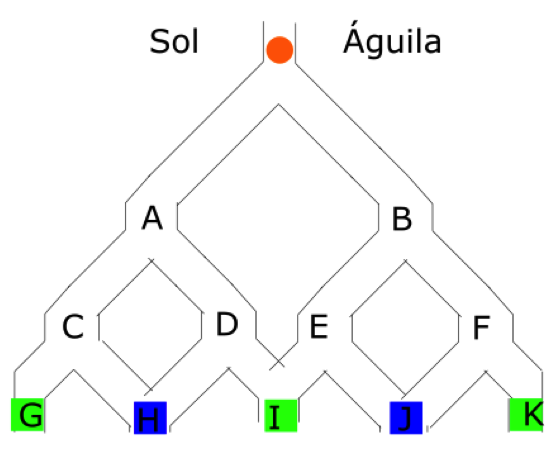
\includegraphics[width=0.4\textwidth]{../images/SINMAT1_U3_AC99_IMG1}
    \caption{Diagrama de \'arbol con todos los posibles resultados del experimento.}
    \label{fig:SINMAT1_U3_AC99_IMG1}
\end{figure}

\begin{parts}
    \part \include*{../parts/question099a01}
    \part \include*{../parts/question099a02}
    \part \include*{../parts/question099a03}
    \part \include*{../parts/question099a04}
    \part \include*{../parts/question099a05}
    \part \include*{../parts/question099a06}
    \part \include*{../parts/question099a07}
\end{parts}